\documentclass[conference, 10pt]{IEEEtran}
\IEEEoverridecommandlockouts

% packages
\usepackage{parskip}
\usepackage{booktabs}
\usepackage{multirow}
\usepackage{cite}
\usepackage{hyperref}
\usepackage{listings}
\usepackage{amsmath,amssymb,amsfonts,amsthm}
\usepackage{algorithmic}
\usepackage{graphicx}
\usepackage{textcomp}
\usepackage{xcolor}
\usepackage{enumitem}
\usepackage{tikz}
\usepackage{footnote}
\usepackage{caption}  % Add this package
\captionsetup{labelfont={bf},textfont=md}

\usetikzlibrary{positioning, shapes, arrows.meta}

\begin{document}

\title{
  {\LARGE WIP: DiLoCo-SWARM: Early steps towards low-communication horizontally scalable decentralized training}
}

\author{
  \IEEEauthorblockN{\bf Mika Senghaas\IEEEauthorrefmark{1}}
  \IEEEauthorblockA{EPFL \\ \textit{mika.senghaas@epfl.ch}}  
  \and
  \IEEEauthorblockN{\bf Martijn De Vos\IEEEauthorrefmark{2}}
  \IEEEauthorblockA{EPFL \\ \textit{martijn.devos@epfl.ch}}
  \and
  \IEEEauthorblockN{\bf Rishi Sharma\IEEEauthorrefmark{2}}
  \IEEEauthorblockA{EPFL \\ \textit{rishi.sharma@epfl.ch}}
  \and
  \IEEEauthorblockN{\bf Akash Dhasad\IEEEauthorrefmark{2}}
  \IEEEauthorblockA{EPFL \\ \textit{akash.dhasade@epfl.ch}}
}

\maketitle

{\small\itshape \IEEEauthorrefmark{1} Author, \IEEEauthorrefmark{2} Supervisor}

\begin{abstract} 
  ...
\end{abstract}

\begin{IEEEkeywords}
Decentralized Training, DiLoCo, SWARM
\end{IEEEkeywords}

\section{Introduction} 

% Scale
Following the promises of the scaling laws~\cite{kaplan2020,hoffmann2022},
modern foundation models have hundreds of billion of parameters and are trained
on tens of trillions of
tokens~\cite{brown2023,touvron2023,dubey2024,openai2024,chowdhery2022,geminiteam2024}.
At this scale, it is infeasible to train on a single device. A natural solution
is to distribute computation, i.e. have many devices collaboratively train a
single model.

% Distributed training
The main idea in distributed training is to partition the data, model, and
optimiser states across devices to lower the memory usage per device and
training time through parallel computation. Many parallelisation techniques have
been proposed, most notably data parallelism, pipeline parallelism , and tensor
parallelism. Often, models use these techniques in conjunction~\cite{dubey2024,
shoeybi2020}. For example, Llama 3.1 405B employs four types of parallelism
across 16K H100 GPUs~\cite{dubey2024}. However, naive implementations of these
techniques only work well under the assumption of fast, homogeneous compute, as
present in data centers. Hence, training frontier models is currently restricted
to those with access to multi-million dollar compute clusters. 

% Decentralization
Decentralization is a promising alternative that is based on the idea of utilizing
vast cheap, consumer-grade resources that are distributed across the globe. In this
paradigm, volunteers could donate idle compute and collaboratively train the next
generation of democratic, open-source foundation models. While appealing, this vision
is not yet reality because of a lack of efficient algorithms for fully decentralized
training.  

% SOTA Decentralized training
To this date, the largest decentrally trained model is
Intellect-1~\cite{intellect1}, a 10B parameter model trained on 1 trillion
tokens using up to 14 concurrent nodes across three continents. Intellect-1 is a
scale-up of DiLoCo~\cite{douillard2023}, a distributed data parallel training
framework which reduces communication requirements by a large factor without
sacrificing performance. This training run marks a milestone in decentralized
training, but, as is, the method is not scalable to compete with models trained
in a centralized setting. The main reason is that, at its core, DiLoCo is still
a data parallel method, which requires each worker to hold a copy of the entire 
model and local optimizer states. For example, during the training of Intellect-1,
the minimum requirement for each worker were 8xH100 GPUs, prohibitive for most 
volunteer compute. 

% SWARM
SWARM~\cite{ryabinin2023} is a promising, but less explored, alternative that
interpolates data and pipeline parallelism in the decentralized setting. By sharding
the model, SWARM is able to scale to larger models, or vice versa, allow
lower-end devices to participate in training. Through a dynamic pipelining approach,
SWARM is able to find optimal trajectories through redundant workers in pipeline stages,
and allows for 2D parallelism in a decentralized setting with failures.

The original SWARM algorithm has only been tested in the original implementation,
and also its publicly hosted inference variant, Petals~\cite{borzunov2023}, does 
not have any active compute contributors or maintainers.

% Contributions
This work aims to kick-off an open-source effort to re-implementing SWARM, making
it accessible and attractive for the community to use and continue research on decentralized training. To this end, this work makes the following two significant contributions:

\begin{enumerate}
  \item \textbf{Implementation} A minimal PyTorch-only implementation of a feature-subset of SWARM which runs Single-GPU, data parallel, pipeline parallel and SWARM-style training, optionally using DiLoCo-style training.
  \item \textbf{Diloco-SWARM} We show that SWARM is compatible with DiLoCo-style training, and ... % TODO: Add details of resuls
\end{enumerate}

% Open-source resources
We open-source the full experiment code and results on \href{https://github.com/mikasenghaas/swarm}{GitHub} and \href{https://wandb.ai/mikasenghaas/swarm}{Weights \& Biases}, as well as a distilled version of the training script as a \href{https://gist.github.com/mikasenghaas/5fa1aa77ea69f187f531a5889983c249}{GitHub Gist}. We hope that these resources will be useful for the community to continue research on decentralized training
and accelerate the democratization of AI.

\section{Background}
\label{sec:background}

% TODO: Add figure visualizing DiLoCo, SWARM, and DiLoCo-SWARM

% Challenges in decentralized training
% \begin{enumerate}[label=(\arabic*)]
%   \item (\textit{Network}) Devices may be distributed globally; an efficient
%     algorithm trains efficiently despite slow interconnect
%   \item (\textit{Hardware}) Devices may range from consumer-grade to
%     data centre GPUs; an efficient algorithm  ensures high utilisation across
%     all devices
%   \item (\textit{Reliability}) Devices may leave or enter the training at any
%     time; a robust algorithm is fault-tolerant and dynamically adapts to the
%     amount of compute available
%   \item \textit{(Scale)} Devices may be numerous; a scalable method should be
%     more efficient as more compute becomes available, independent of the model or
%     data size
% \end{enumerate}


\subsection{DiLoCo}
\label{subsec:diloco}

Stochastic gradient-based training naturally lends itself to an easy form of
parallelism, called data parallelism. Here, each worker holds a copy of the
entire model and a local data shard. Each device trains locally, before the local
gradients are synchronised. Traditional data parallel methods~\cite{mcmahan2016}
require synchronisation of local gradients at every step, rendering the method
unfeasible in a decentralised setting as communication costs are too high.

% DiLoCo
DiLoCo~\cite{douillard2023} is a framework that enables low-bandwidth data
parallel training on poorly connected islands of workers. It proposes an
inner-outer optimisation scheme, in which workers train for $H\sim 500$ steps on
local data shards using AdamW~\cite{loshchilov2019} before synchronising
pseudo-gradients using a global Nesterov optimiser. DiLoCo sets the standard for
distributed data parallel training, matching performance of traditional methods
while significantly reducing wall clock-time and communication cost. While
DiLoCo is robust to dynamic worker arrangements, it faces many of the same
challenges as traditional data parallel training. In particular, the synchronous
nature of the global gradient update can lead to significant idle time when
faster workers have to wait for slower workers to finish their local training
task. Further, DiLoCo does not scale naturally to huge models that do not fit
into the workers' memory - relying on slow parameter offloading
methods~\cite{rhu2016, cui2016} to scale.

% Asynchronicity in DiLoCo
Follow up work from DeepMind~\cite{li2024} tries to address the efficiency
issues in heterogeneous environments by allowing asynchronous global updates on
a centralised parameter server. While comprehensive, the work does not find a
scalable solution to asynchronous data parallel training yet.

\subsection{SWARM}
\label{subsec:swarm}

% Pipeline parallelism
When a single worker cannot fit the entire model into memory, the model itself
has to be sharded. A common technique is pipeline parallelism which partitions a
model vertically into groups of subsequent layers. In this paradigm, activations
need to be communicated between workers handling subsequent layers during the
forward, and gradients during the backward pass. Traditional pipeline
parallelism is not feasible in the decentralised setting. Due to its inherently
sequential nature, the entire pipeline is bottlenecked by its weakest link,
leading to idle time for quicker workers. Furthermore, a naive implementation is
not fault-tolerant, as the failure of any worker will stall the entire training
procedure.

% SWARM
SWARM parallelism~\cite{ryabinin2023} translates the idea of pipeline
parallelism into an efficient algorithm in the distributed setting. Their main
innovation is in constructing a dynamic and redundant pipeline: each pipeline
stage is served by a swarm of devices. Any device in a swarm may communicate
with any device in the preceding and succeeding stage. They introduce
\textit{stochastic wiring} where each device makes a request to the next
pipeline stage according to statistics on the throughput of the available
devices, ensuring that faster or better connected devices handle more requests.
Further, due to \textit{swarm balancing}, devices periodically switch from
under- to overutilised swarms to distribute the workload. In theory, any worker
that can hold a (small) shard of the model in memory can participate in SWARM. 
High latency and high dropout rates in the network increase training time, but 
stochastic wiring and adaptive swarming helps to find optimal trajectories
through the pipeline stage, even under suboptimal conditions. SWARM naturally
satisfies on- and off-ramping of devices during training, and the algorithm is
naturally fault-tolerant due to its redundant design. In summary, SWARM was
designed from first principles to be robust and effective in the decentralised
setting considered in this work.

% Genetic scheduling
% Finally, Yuan et. al~\cite{yuan2022} try to combine data and pipeline
% parallelism by finding an optimal allocation of devices to micro-batches and
% pipeline stages such that the global communication requirements are minimised.
% They propose a genetic algorithm that jointly minimises communication
% requirements. Yet, their global scheduling is static and, consequently, does not
% handle device failures.
% 
% % Complementary research directions
% Many works also consider complementary approaches to decrease communication
% requirements, for example by gradient sparsification, quantisation or delayed
% parameter updates~\cite{yuan2022, ryabinin2023, tang2020}.

\section{Method}
\label{sec:method}

We introduce a new algorithm, DiLoCo-SWARM, that combines DiLoCo and SWARM.

% Describe the algorithm (take inspiration from DiLoCo and SWARM) paper

\section{Implementation}
\label{sec:implementation}

% Detail algorithm

\section{Experiments}
\label{sec:experiments}

% Introduction
In this section we report the main experiments validating DiLoCo-SWARM. The experiment
mostly follows the setup and hyper-parameters of DiLoCo~\cite{douillard2023}.

% Dataset
We consider a language modeling task on the FineWeb-Edu~\cite{penedo2024}
dataset, a large pre-training dataset consisting of high-quality web pages
filtered for educational content. We choose this dataset over other common
pre-training datasets, such as C4~\cite{}, due to its high token efficiency
allowing to surpass GPT-2~\cite{radford2019} on the HellaSwag~\cite{zellers2019}
benchmark with 10x less data~\cite{karpathy2024}.

% Main Experiment: DiLoCo-SWARM
For our main experiment, we train three GPT-2 (124M) models from scratch, two
baselines and one DiLoCo-SWARM:

\begin{enumerate}
  \item \textbf{Weak Baseline} (Single GPU): The weak baseline trains for 2,000
  steps on a single GPU with a batch size of 512 and sequence length of 1024,
  for a total training budget of 1B tokens. 
  \item \textbf{Strong Baseline} (SWARM): The strong baseline is a 4x2 SWARM,
  i.e. four workers in two pipeline stages, which does regular SWARM training
  with gradient synchronization after every step. The higher compute budget is
  used to scale the batch size to the number of worker per stage, leading to a
  total training budget of 4B tokens. Note, that in theory, SWARM can train a
  model double the size of the baseline as its parameters and optimzer states
  are sharded across pipeline stages, leading to a total model size that scales
  with the number of stages. 
  \item \textbf{DiLoCo-SWARM}: The final model is a 4x2 DiLoCo-SWARM, which uses
  the same setup and compute budget as the SWARM baseline but communicates
  gradients only every $H$ steps.
\end{enumerate}

The hyperparameters for the run are identical to those in
DiLoCo~\cite{douillard2023}. The inner optimizer is initialized to AdamW with a
learning rate of $10^{-4}$, and a weight decay of $0.01$. In DiLoCo-SWARM, the
outer optimizer is initialized to Nesterov with a learning rate of $0.7$ and a
momentum of $0.9$. The learning rate is warmed up linearly over 50 steps and the
synchronization frequency is set to 50 inner steps, which is scaled down to
proportionally match the values found in the DiLoCo~\cite{douillard2023}
experiments. A detailed description of the hyperparameters is provided in
Table~\ref{tab:hyperparameters} in the Appendix.

% Experiment 2: DiLoCo Comparison
Next, we compare DiLoCo to DiLoCo-SWARM. To this end, we replicate the DiLoCo
experiments and train a strong DDP baseline and a DiLoCo instance on 8x the
batch size. 

% Experiment 3: Ablation on communication frequency

% Experiment 4: Ablation on data distribution (IID vs. non-IID)

% Evaluation
For all experiments, our main evaluation metric is the perplexity on the
validation set. We evaluate on a randomly sampled, but constant validation split
containing 10M tokens throughout training to show the convergence against the
number of training steps, and wall-clock time.

\section{Results}
\label{sec:results}

\begin{figure*}[t!]
  \centering
  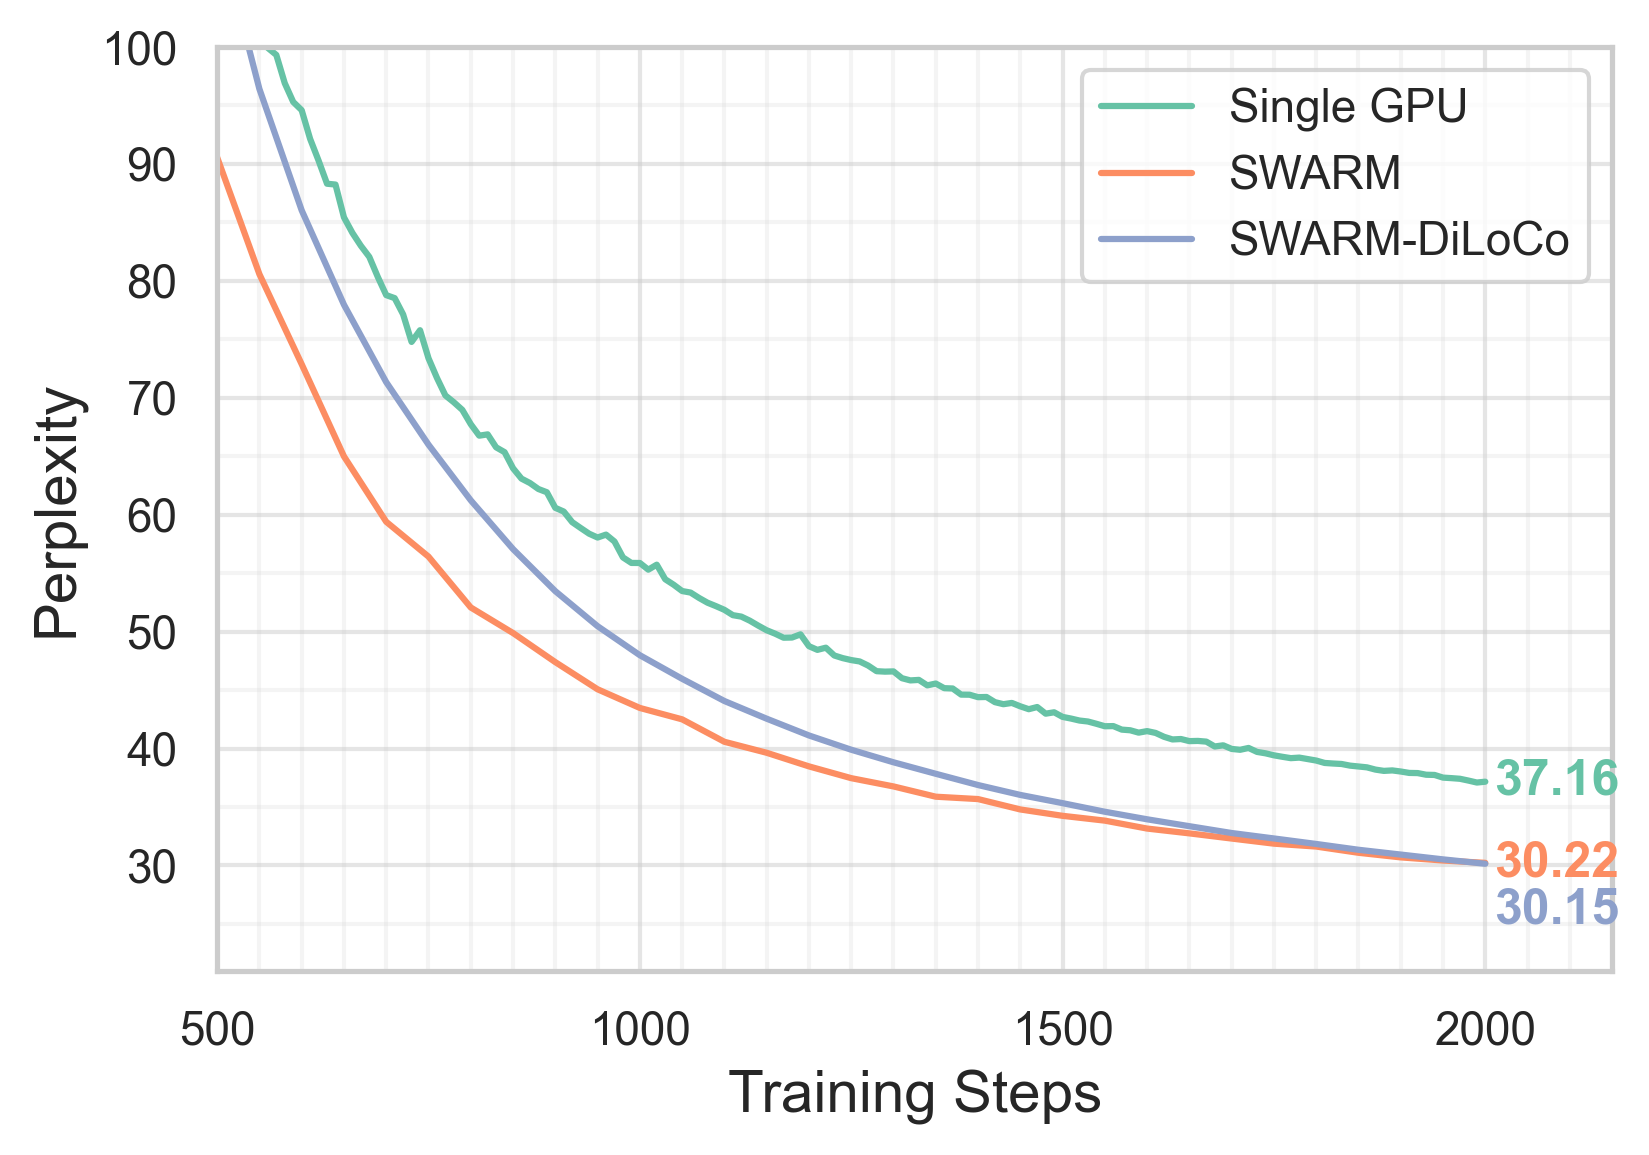
\includegraphics[width=0.8\textwidth]{figures/experiment1.png}
  \caption{}
  \label{fig:experiment1}
\end{figure*}

\begin{figure}[t!]
  \centering
  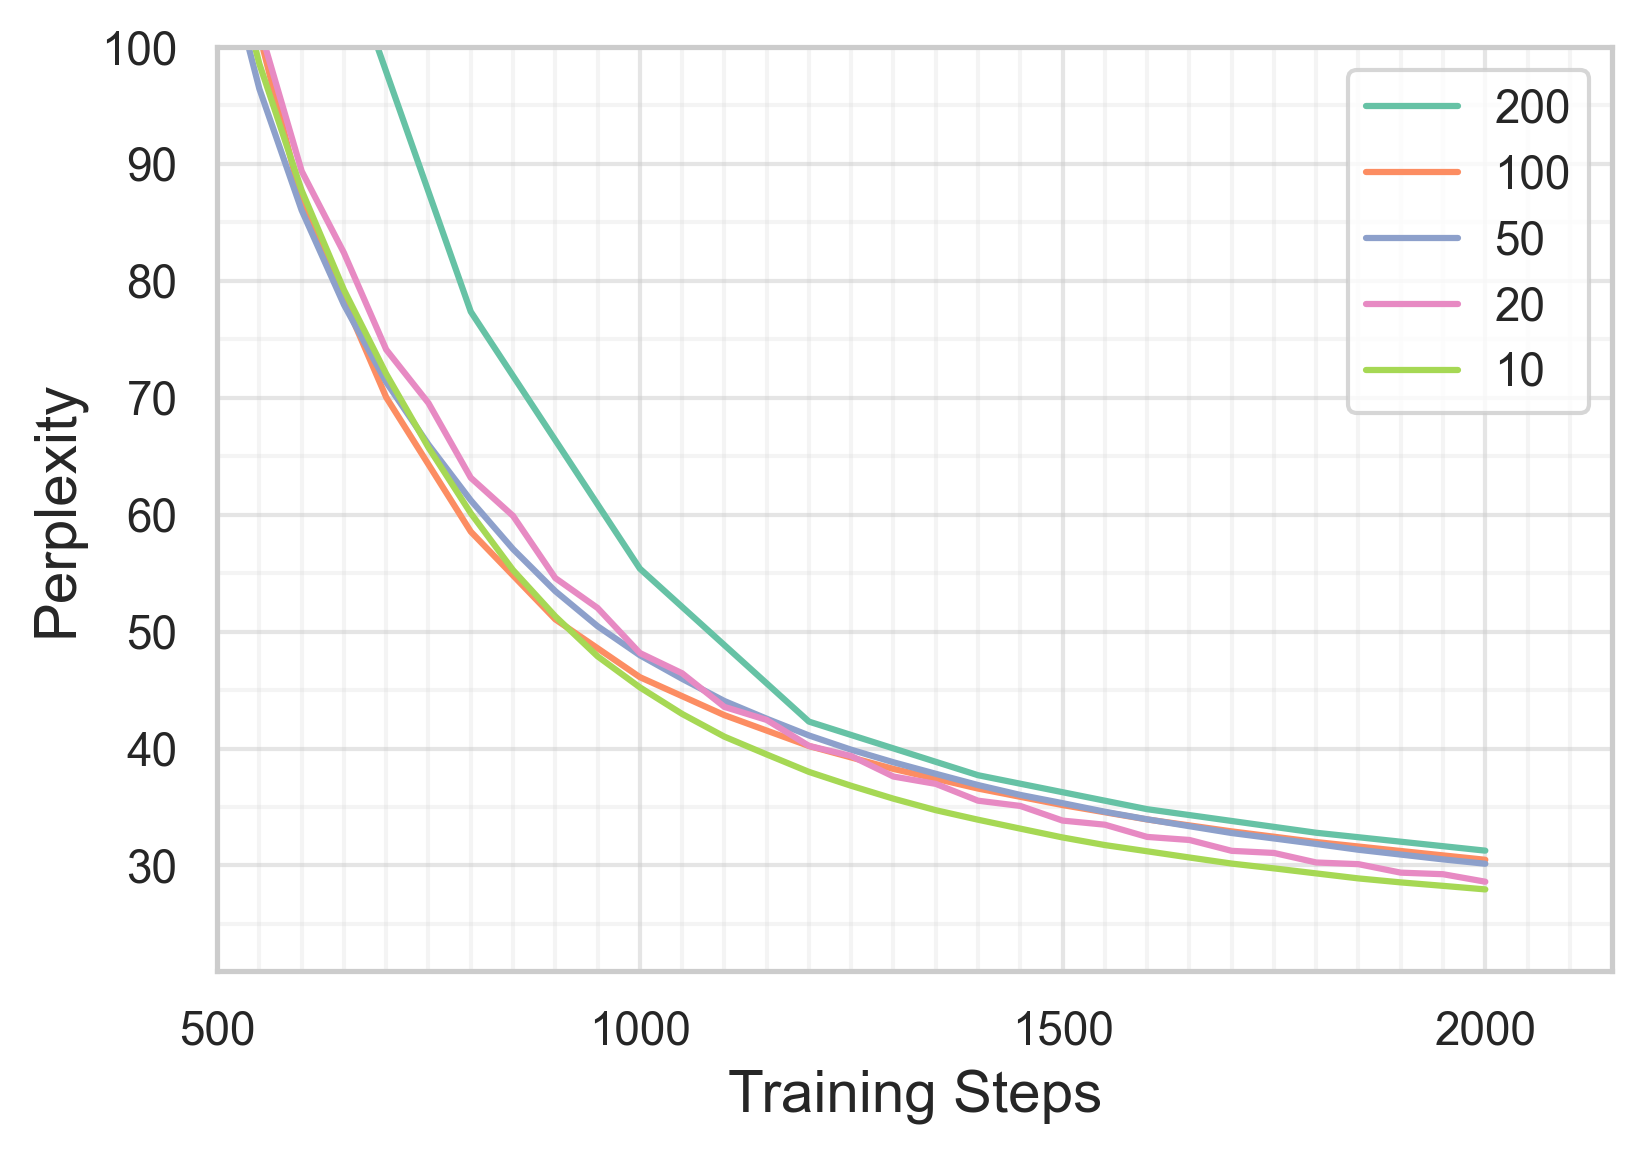
\includegraphics[width=\linewidth]{figures/experiment2.png}
  \caption{}
  \label{fig:experiment2}
\end{figure}

% TODO: Add results

\begin{table*}[t!]
  \centering
  \begin{tabular}{l|cccccc}
  \toprule
  Model & Gradient Sync & Time & Compute & Data & Model Size \\
  \midrule
  \textbf{Single GPU} (\textit{Weak Baseline}) & 0 & 1$\times$ & 1$\times$ & 1$\times$ & 1$\times$ & - \\
  \textbf{SWARM} (\textit{Strong Baseline}) & 4$\times N$ & 1$\times$  & 8$\times$ & 4$\times$ & 2$\times$ & - \\
  \textbf{DiLoCo-SWARM} & 4$\times N/H$ & 1$\times$ & 8$\times$ & 4$\times$ & 2$\times$ & - \\
  \bottomrule
  \end{tabular}
  \caption{Main Experiment Results}
  \label{tab:main-results}
\end{table*}


\section{Limitations}
\label{sec:limitations}

% No hyperparameter tuning over SWARM-DiLoCo hyper-parameters
% Relatively small scale model and data (DiLoCo experiments train for 88k steps on 150M, OpenDiLoCo train for 88k steps on up to 1B)


\section{Discussion}
\label{sec:discussion}

\subsection{Summary}
\label{subsec:summary}

\subsection{Future work}
\label{subsec:future-work}

\subsection{Acknowledgements}
\label{subsec:acknowledgements}

This work was developed in collaboration with the Scalable Computing Systems
(SaCS) lab at EPFL as well as Prime Intellect. All compute was kindly sponsored
by Prime Intellect.

\bibliography{references}
\bibliographystyle{IEEEtran}

\appendix

% Hardware
\textbf{Hardware.} All experiments were conducted on a single node with eight
co-located H100 GPUs on the \href{https://app.primeintellect.com/}{Prime
Intellect Compute} platform.

% Hyperparameters
\textbf{Hyperparameters.} Table~\ref{tab:hyperparameters} shows the
hyperparameters used in the experiments. The outer optimizer parameters is only
used for DiLoCo-style training, else the outer optimization simply synchronizes
the inner model gradients before performing a regular update.

\begin{table}[h]
\centering
\begin{tabular}{llc}
\toprule
\textbf{Hyperparameter} & \textbf{Value} \\ 
\midrule
\multirow{1}{*}{General} & Batch Size & 512 \\ 
& Sequence Length & 1024 \\ 
& Steps & 2000 \\
\hline
\multirow{1}{*}{InnerOptimizer} & Name & AdamW \\ 
& Weight decay & - \\ 
& Learning Rate & $4 \times 10^{-4}$ \\ 
\hline
\multirow{1}{*}{OuterOptimizer} & Name & Nesterov \\ 
& Learning Rate & 0.7 \\ 
& Momentum & 0.9 \\ 
\bottomrule
\end{tabular}
\caption{Hyperparameters}
\label{tab:hyperparameters}
\end{table}


\end{document}
